\documentclass{article}

\usepackage{graphicx}
\usepackage{blindtext}
\usepackage{wrapfig}
\usepackage[backend=biber]{biblatex}
% \usepackage{biblatex}

\addbibresource{MyDoc.bib}

\author{zhuangyulin}
\title{haha}


\begin{document}
\maketitle

\section{Introdution let go}

here is a new document.

So in \ref{list}, we will see list.

So emasc is in number \ref{remacs}.

\section{Text format}
This is normal text. 

\textbf{This is BOLD.}

\textit{This is italic.}

\emph{This is emphatic.}

\underline{Here is underline.}

"This is quote sth"
``This is quote sth''
`This is quote sth'

\section{Lists\label{list}}
\subsection{ordered list}
\begin{enumerate}
    \item vim
    \item emacs \label{remacs}
    \item vscode
\end{enumerate}

\subsection{unordered list}
\begin{itemize}
    \item vim
        \begin{itemize}
            \item vim8
            \item neovim
        \end{itemize}
    \item emacs
    \item vscode
\end{itemize}


\section{Labels}




\section{See images}
\begin{center}
    
\includegraphics[width=0.7\textwidth,angle=90]{arch.png}
\end{center}

\blindtext
This figure show us.

\begin{figure}
    \centering
    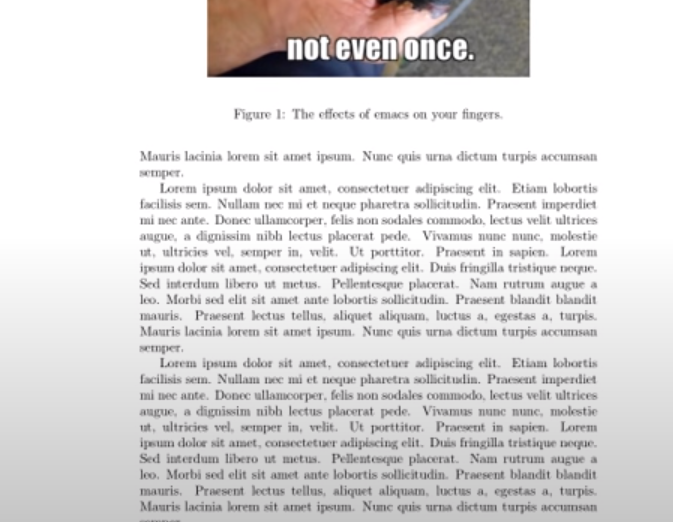
\includegraphics[width=0.7\textwidth,angle=90]{book.png}
    \caption{book for us}
\end{figure}

\blindtext

\blindtext

\blindtext

\subsection{wrap figure}

\begin{wrapfigure}{r}{3in}
    \centering
    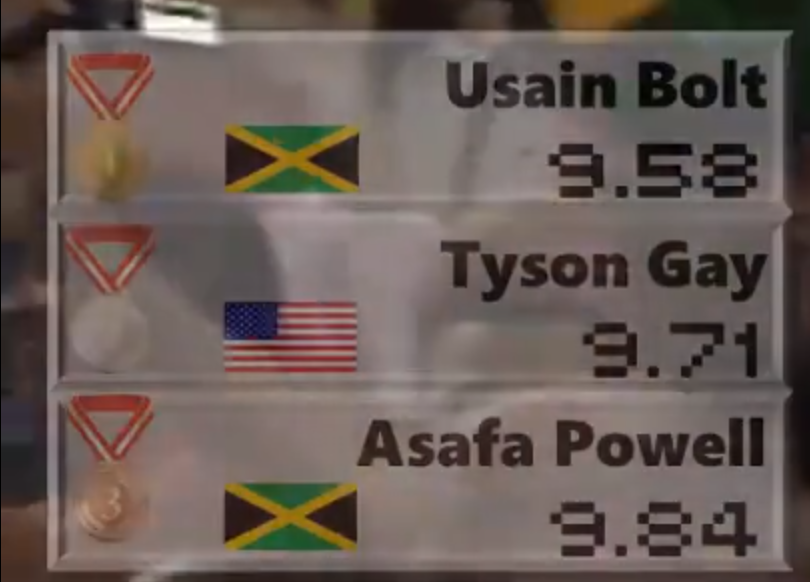
\includegraphics[width=2.5in]{bolt.png}
    \caption{bolt 100}
\end{wrapfigure}


\section{Bibliography management}

As \cite{arbelaez2011contour} says, it is shit.  

% \bibliography{MyDoc.bib}
\printbibliography

\end{document}

